\section{ОКРУЖНОСТЬ И КРУГ}
\pagestyle{plain}

\textbf{2017.} Углы $NBA$ и $NMB$ являются вписанными в окружность и опираются на две дуги, которые в сумме составляют половину окружности. Поэтому сумма этих углов равна $90^\circ$. Тогда $\angle NMB = 90^\circ - \angle NBA = 19^\circ.$ \newline \null \hspace*{\fill} Ответ: 19.

\textbf{2018, 2019} $-$ аналогичные задачи.

\textbf{2020.}

{\centering 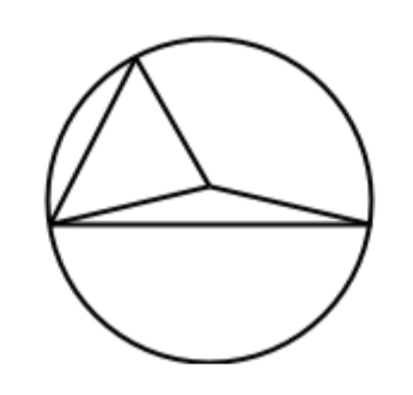
\includegraphics[width=0.4\linewidth]{Geometry/Content/33.png}
	
}

Соединим центр окружности с точкой $B$. Тогда $OA=OB= \linebreak = OC$ как радиусы, треугольники $OAB$ и $ODC$ $-$ равнобедренные, т.е. $\angle OBA = \angle OAB = 53^\circ$, а $\angle BCO = \angle OBC$. Но $\angle OBC = \linebreak=\angle ABC - \angle OBA = 62^\circ - 53^\circ = 9^\circ.$ \newline \null \hspace*{\fill} Ответ: 9.

\textbf{2021, 2022} $-$ аналогичные задачи.

\textbf{2023.} Длина дуги окружности пропорциональна величине центрального угла, опирающегося на эту дугу. Поэтому $\frac{l_1}{l_2} = \frac{\alpha_2}{\alpha_2}$, где $l_1$, $l_2$ - меньшая и большая длины дуг $AB$, $\alpha_1 = 45^\circ$, $\alpha_2 = \linebreak=360^\circ - 45^\circ = 315^\circ$. Тогда $l_2 = \frac{l_1 \alpha_2}{\alpha_1} = \frac{91\cdot 315}{45} = 637$. \newline \null \hspace*{\fill} Ответ: 637.

\textbf{2024, 2025} $-$ аналогичные задачи.

\textbf{2026.} Сторона квадрата, описанного около окружности, равна ее диаметру, т.е. $a = 2R = 28$. Площадь квадрата $S = a^2 = 784$. \newline \null \hspace*{\fill} Ответ: 784.

\clearpage 

\textbf{2027, 2028} $-$ аналогичные задачи.

\textbf{2029.} В равнобедренном $\Delta ABC$ $\angle A = \frac{180^\circ - 88^\circ}{2} = 46^\circ$, а центральный угол $BOC$ опирается на ту же дугу, что и вписанный в окружность $\angle A$. Поэтому он в два раза больше и равен $92^\circ$. \newline \null \hspace*{\fill} Ответ: 92.

\textbf{2030, 2031} $-$ аналогичные задачи.

\textbf{2032.} $\angle ACB = \frac{\angle AOB}{2} = 57,5^\circ$. \newline \null \hspace*{\fill} Ответ: 57,5.

\textbf{2033, 2034} $-$ аналогичные задачи.

\textbf{2035.} $\Delta BOC$ $-$ равнобедренный, т.к. $OB=OC$ (как радиусы). $\angle BOC = \angle AOD = 44^\circ$ как вертикальные углы. Тогда $\angle ACB = \linebreak = \angle OCB = \frac{180^\circ-44^\circ}{2} = 68^\circ.$ \newline \null \hspace*{\fill} Ответ: 68.

\textbf{2036, 2037} $-$ аналогичные задачи.

\textbf{2038.} Угол $C$, опирающийся на диаметр, равен $90^\circ$. Тогда в прямоугольном $\Delta ABC$ $\angle ABC = 90^\circ - \angle BAC = 57^\circ.$ \newline \null \hspace*{\fill} Ответ: 68.

\textbf{2039, 2040} $-$ аналогичные задачи.

\textbf{2041.} Пусть $\alpha, \beta$ $-$  градусные меры дуг $AD$ и $DC$. Тогда $\newline\angle ABD =  \frac{\alpha}{2} = 38^\circ$, откуда $\alpha = 76^\circ$. Аналогично $\beta = 2 \cdot 54^\circ = 108^\circ$.
Тогда $\angle ABC = \frac{\alpha + \beta}{2} = 92^\circ$. \newline \null \hspace*{\fill} Ответ: 92.

\textbf{2042, 2043} $-$ аналогичные задачи.


\textbf{2044.}

{\centering 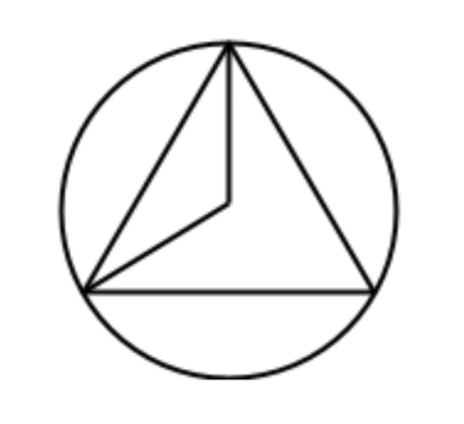
\includegraphics[width=0.4\linewidth]{Geometry/Content/34.png}
	
}

Пусть дана окружность радиуса $R$ с центром в точке $O$ и  вписанный в нее правильный $\Delta ABC$.  Соединим точку $O$ с вершинами $B$ и $C$ и рассмотрим равнобедренный $\Delta OBC$. В нем угол при вершине $O$ в силу симметрии равен $120^\circ$, боковые стороны равны радиусу $R$, а углы при основании равны $30^\circ$. По теореме синусов $\frac{BC}{OC} = \frac{\sin{120^\circ}}{\sin{30^\circ}} = \sqrt{3}$. Отсюда $R = OC = \frac{BC}{\sqrt{3}} = 36$. 

\null \hspace*{\fill} Ответ: 36.

\textbf{Замечание.} В школьном курсе геометрии пользуются соотношением $R = \frac{a}{\sqrt{3}}$ между радиусом окружности $R$ и стороной правильного вписанного треугольника $a$. Фактически в решении задачи \textbf{2044} это соотношение выведено. 

Аналогично решаются задачи \textbf{2045-2049}.

\textbf{2050.}  

{\centering 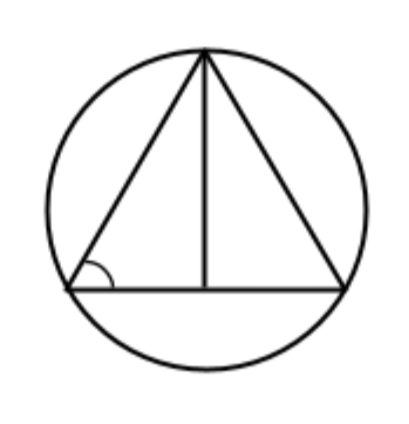
\includegraphics[width=0.4\linewidth]{Geometry/Content/35.png}
	
}

Проведем в равностороннем $\Delta ABC$ высоту $CH \perp AB$. Тогда в прямоугольном $\Delta BCH$ $\frac{CH}{BC} = \sin{60^\circ} = \frac{\sqrt{3}}{2}$, $BC = \frac{2CH0}{\sqrt{3}}$. Радиус описанной окружности $R = \frac{BC}{\sqrt{3}} = \frac{2CH}{3} = \frac{2\cdot 90}{3} = 60.$ \newline \null \hspace*{\fill} Ответ: 60.

Задачи \textbf{2051-2055} решаются аналогично.

\textbf{2056.} Гипотенузу $AB$ найдем по теореме Пифагора:
\[
AB = \sqrt{AC^2+BC^2} = \sqrt{64+225} = 17.
\]
Радиус описанной окружности равен половине гипотенузы, т.е. 8,5. \newline \null \hspace*{\fill} Ответ: 8,5.


Задачи \textbf{2057-2061} решаются на основании аналогичных соображений.

\textbf{2062.} 

{\centering 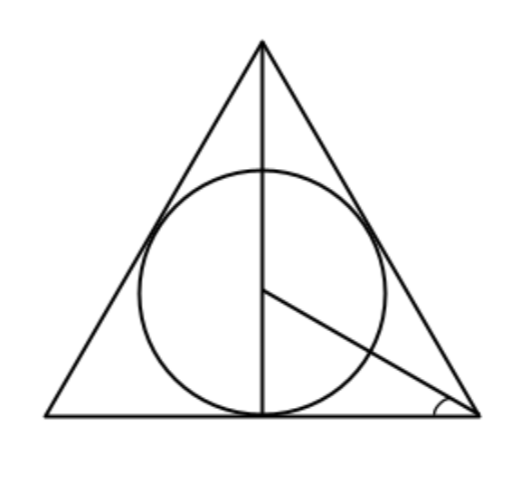
\includegraphics[width=0.4\linewidth]{Geometry/Content/36.png}
	
}

Пусть $ABC$ $-$ правильный треугольник. В силу симметрии центр вписанной и описанной окружностей находится в одной и той же точке $O$, являющейся точкой пересечения высот, медиан и биссектрис данного треугольника. Поэтому $BH=h$ $-$ высота треугольника, $OH$ $-$ радиус вписанной окружности, а $OB=OC =\linebreak= R$ $-$ радиус описанной окружности. Кроме того, т.к. $OC$ $-$ биссектриса, то $\angle OCH = 30^\circ$ и из $\Delta OCH$ следует, что $R = 2r$. Поэтому можно записать систему уравнений
\[
\begin{cases}
	R + r = h \\
	R = 2r
\end{cases},
\]
откуда следует, что $r = \frac{h}{3} = \frac{132}{3} = 44.$ \newline \null \hspace*{\fill} Ответ: 44.

Задачи \textbf{2063-2067}  решаются на основании аналогичных соображений.

\textbf{2068.} Пусть $a$ и $r$ сторона треугольника и радиус вписанной в него окружности.  Из чертежа к задаче \textbf{2062} следует, что 
\[
\frac{r}{a/2}  =tg\;30^\circ = \frac{1}{\sqrt{3}}.
\]  
Отсюда $r = \frac{a}{2} tg \; 30^\circ = \frac{a}{2\sqrt{3}} = \frac{4\sqrt{3}}{2\sqrt{3}} = 2.$ \newline \null \hspace*{\fill} Ответ: 2.

Задачи \textbf{2069-2073}  решаются на основании аналогичных соображений.

\textbf{2074.}

{\centering 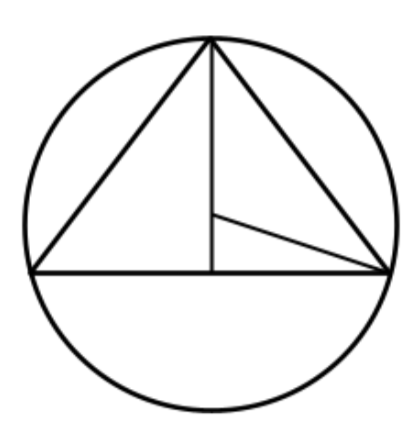
\includegraphics[width=0.35\linewidth]{Geometry/Content/37.png}
	
}

Пусть в $\Delta ABC$ $AB = BC = a = 5$, $AC = b = 6$. В силу симметрии центр описанной окружности $O$ лежит на  высоте (и медиане) $BH$, так что  $OB=OC=R$ $-$ радиус окружности. Высоту $h = BH$ найдем из прямоугольного $\Delta BCH$: $h = \sqrt{a^2-\left( \frac{b}{2} \right)^2} = \linebreak=\sqrt{25-9} = 4$. Тогда в прямоугольном $\Delta OCH$ $OH = h - R$ и по теореме Пифагора $(h - R)^2 + \left( \frac{b}{2} \right)^2 = R^2$, откуда находим $R = \frac{h^2  =\frac{b^2}{4}}{2h} = \frac{25}{8} = 3,125.$ \newline \null \hspace*{\fill} Ответ: 3,125.

\textbf{Замечание.} Можно вычислить площадь $\Delta ABC$: $S = \frac{bh}{2}=12$, а радиус 
найти по известной формуле $R = \frac{abc}{4S} = \frac{5\cdot6\cdot5}{48} = 3,125$.

\textbf{2075, 2076} $-$ аналогичные задачи.

\textbf{2077.}

{\centering 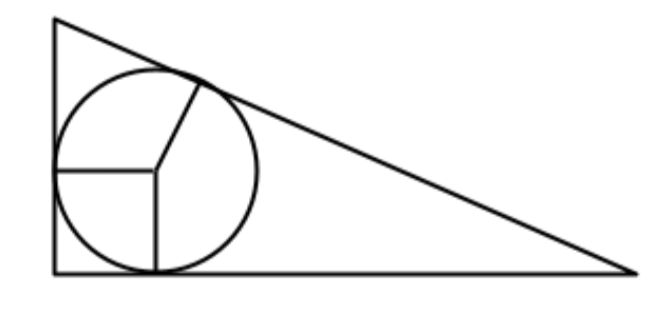
\includegraphics[width=0.5\linewidth]{Geometry/Content/38.png}
	
}

Обозначим  катеты треугольника $BC = a= 4$, $AC = b = 7,5$. Тогда гипотенуза $AB = c = \sqrt{a^2 + b^2} = 8,5$.  Пусть $O$ $-$ центр вписанной окружности радиуса $r$, а $M$, $N$, $P$ точки касания окружности сторон треугольника. Тогда $ON = OP = r$. Т.к. радиусы, проведенные в точки касания, перпендикулярны касательным, четырехугольник $ONCP$ является квадратом, следовательно $CP = CN = r$, $BP = a - r$, $AN = b - r$. По свойству касательных, проведенных к окружности из одной точки, можно записать: $BM = BP = a- r$, $AM = AN = b - r$. Таким образом, $AB = c = a + b - 2r$. Отсюда $r = \frac{a + b - c}{2} = 1,5$.

 \null \hspace*{\fill} Ответ: 3,125.

\textbf{2078, 2079} $-$ аналогичные задачи. 

\textbf{2080.} См. замечание к решению задачи \textbf{2077}.   Полупериметр \linebreak$p = \frac{a+b+c}{2} = \frac{569+569+462}{2}=800$, а площадь треугольника находится по формуле Герона:
\[
S = \sqrt{p(p-a)(p-b)(p-c)} = \sqrt{800\cdot231\cdot231\cdot338} = 120120,
\]
так что $r = \frac{S}{p} = \frac{120120}{800} = 150,15.$ \newline \null \hspace*{\fill} Ответ: 150,15.

\textbf{2081, 2082} $-$ аналогичные задачи.

\textbf{2083.}

{\centering 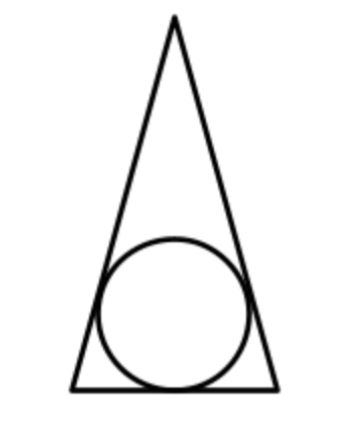
\includegraphics[width=0.35\linewidth]{Geometry/Content/39.png}
	
}

Пусть $ABC$ $-$ равнобедренный треугольник, а $M$, $N$, $P$ $-$ точки касания вписанной окружности сторон треугольника. По свойствам касательных и из соображений симметрии: $BM = BP = 9$, $CM = CN = AN = AP = 1$. ТОгда периметр $P = AB + AC + \linebreak+BC = (9 + 1) + (9 + 1) + (1 + 1) = 22.$ \newline \null \hspace*{\fill} Ответ: 22.

\textbf{2084, 2085} $-$ аналогичные задачи.

\textbf{2086.} Найдем диагональ прямоугольника: $d = \sqrt{a^2+b^2} = \linebreak = \sqrt{225+175} = 20$.  Диагональ является диаметром описанной окружности, а радиус равен 10. \newline \null \hspace*{\fill} Ответ: 10.

Задачи \textbf{2087-2091} решаются из тех же соображений.

\textbf{2092.} Если сторона квадрата $a = 27\sqrt{2}$, то его диагональ $d=\linebreak=a\sqrt{2}=54$ и она является диаметром описанной окружности. Радиус равен 27. \newline \null \hspace*{\fill} Ответ: 127.

Из этих же  соображений решаются задачи \textbf{2093-2097}.

\textbf{2098.} Для ромба (как и для любого выпуклого многоугольника, в который можно вписать окружность) справедлива формула $S = rp$, выражающая связь площади $S$ с полупериметром $p$ и радиусом вписанной окружности $r$.

Если задана сторона ромба $a=34\sqrt{3}$ и угол между сторонами $\alpha = 60^\circ$, то $S = a^2 \sin{\alpha},$ $p = 2a$ и $r = \frac{S}{p} = \frac{a\sin{\alpha}}{2}=\frac{34\sqrt{3}\cdot\frac{\sqrt{3}}{2}}{2} = 25,5$.

\null \hspace*{\fill} Ответ: 25,5.

 Эти же соображения следует использовать при решении задач \textbf{2099-2103}.
 
 \textbf{2104.} Если в трапецию вписана окружность радиуса $R$, то высота трапеции $h$ равна диаметру окружности, т.е. $h = 2R = \linebreak = 2\cdot28 = 56.$ \newline \null \hspace*{\fill} Ответ: 56.
 
\textbf{2105, 2106} $-$ аналогичные задачи.

\textbf{2107.}  В силу симметрии в окружность вписать можно только равнобедренную трапецию. Пусть $a$, $b$ и $m = \frac{a+b}{2}$ $-$ основания и средняя линия трапеции, а $l$ $-$ ее боковая сторона. Тогда периметр трапеции $P = a + b+2l = 2m+2l$, откуда $l = \frac{P-2m}{2}=\linebreak =\frac{96-32}{2}=32$. \newline \null \hspace*{\fill} Ответ: 32.

\textbf{2108, 2109} $-$ аналогичные задачи.

\clearpage
\textbf{2110.}

{\centering 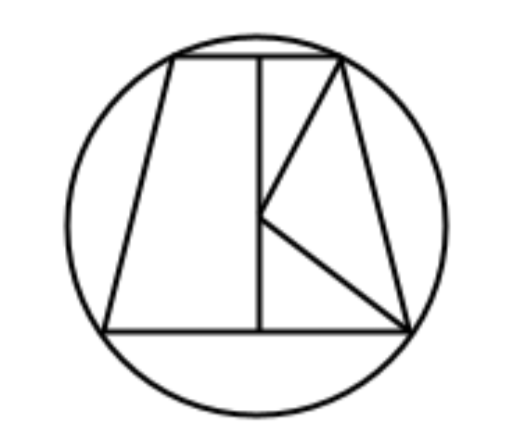
\includegraphics[width=0.35\linewidth]{Geometry/Content/40.png}
	
}

Пусть $ABCD$ $-$ равнобедренная трапеция с основаниями $\linebreak AD = a =48$ и $BC = b = 20$, вписанная в окружность радиуса $R=26$. В силу симметрии центр окружности, т.е. точка $O$, находится на отрезке $MN$, соединяющем середины оснований. Тогда $OC=OD=R$. Отрезок $MN$ является высотой трапеции $h$. Поскольку по условию задачи точка $O$ находится внутри трапеции, то
\begin{eqnarray*}
h=OM+ON=\sqrt{R^2- \left( \frac{b}{2} \right)^2} +\sqrt{R^2- \left( \frac{a}{2} \right)^2} =\\ =\sqrt{676-100} - \sqrt{676-576}=24+10=34.
\end{eqnarray*} \null \hspace*{\fill} Ответ: 34.

\textbf{2111, 2112} $-$ аналогичные задачи.

\textbf{2113.}

{\centering 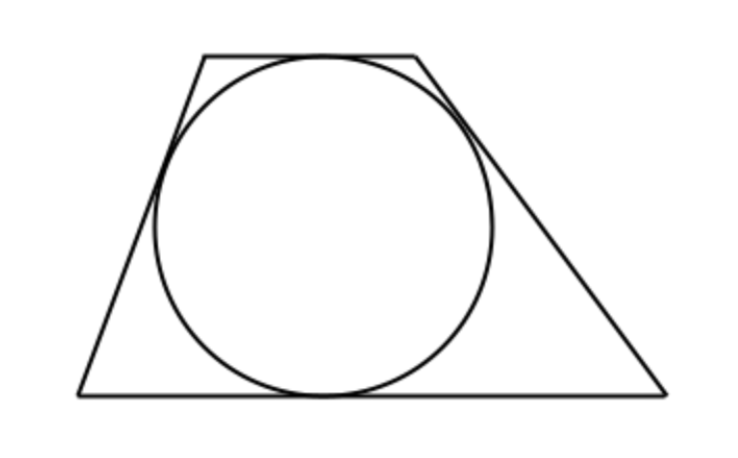
\includegraphics[width=0.4\linewidth]{Geometry/Content/41.png}
	
}

 Пусть трапеция $ABCD$ описана около окружности. Точки касания $M$, $N$, $P$, $Q$. 
  
Докажем известный из школьной геометрии факт: если трапеция описана около окружности, то сумма длин оснований равна сумме длин ее боковых сторон.

Будем использовать свойство двух касательных, проведенных к окружности из одной точки $К$:   длины касательных (от точки $К$ до точек касания) равны. Поэтому (см. чертеж):
\[
BN=BP\;\;CP=CQ\;\;DQ=DM\;\;AM=AN.
\]
Но сумма длин оснований равна $AM+DM+BP+CP$, а сумма длин боковых сторон есть $AN+BN+CQ+DQ$. С учетом приведенных равенств эти суммы совпадают.

В нашем случае  сумма боковых сторон равна 19, сумма оснований также равна 19, тогда средняя линия равна 9,5. \newline \null \hspace*{\fill} Ответ: 9,5.

\textbf{Замечание.} Приведенные выше соображения можно распространить на \textbf{любой выпуклый четырехугольник}, в который вписана окружность: в таком четырехугольнике суммы длин противоположных сторон равны. 

Отсюда же следует, что в прямоугольник (если это не квадрат) и в параллелограмм (если это не ромб) \textbf{вписать окружность нельзя}.  

Приведенные соображения следует использовать при решении задач \textbf{2114-2118}.

\textbf{2119.} Эта задача легко решается без чертежа. Если трапеция прямоугольная, то меньшая боковая сторона равна диаметру вписанной окружности, т.е. $2R$. Сумма боковых сторон равна сумме оснований, т.е. половине периметра $P$. Поэтому $2R+35=\frac{P}{2}=50$. Отсюда $2R=15$, $R=7,5$. \newline \null \hspace*{\fill} Ответ: 7,5.

\textbf{2120, 2121} $-$ аналогичные задачи.

\textbf{2122.} С учетом замечания к решению задачи \textbf{2113} можно утверждать, что периметр четырехугольник равен $2\cdot(17+22)=78$. \newline \null \hspace*{\fill} Ответ: 78.

\textbf{2123, 2124} $-$ аналогичные задачи.

\textbf{2125.} Здесь тоже чертеж не нужен. Поскольку периметр $P=26$, $\frac{P}{2}=13$, а сумма данных сторон не равна 13, то речь идет о двух \textbf{смежных} сторонах. Стороны, противоположные данным, \clearpage имеют длины: $13-5=8$ и $13-9=4$. \newline \null \hspace*{\fill} Ответ: 8.

\textbf{2126, 2127} $-$ аналогичные задачи.

\textbf{2128.} $AB+CD=AD+BC$, $AD=AB+CD-BC=7+9-12=4.$ \newline \null \hspace*{\fill} Ответ: 4.

\textbf{2129, 2130} $-$ аналогичные задачи.

\textbf{2131.} Обозначим три стороны, отношения которых заданы, через $x$, $5x$, $9x$. Если стороны перечислены в последовательном порядке, то это означает, что противоположные стороны $x$ и $9x$. Сумма их длин равна $10x$, такой же должна быть и сумма двух других сторон. Следовательно, длина четвертой стороны равна $10x-5x=5x$. Сумма длин всех четырех сторон, т.е. $20x$, равна периметру $P=20$. Таким образом, $x=1$, а большая сторона $9x=9$. \newline \null \hspace*{\fill} Ответ: 9.

\textbf{2132, 2133} $-$ аналогичные задачи.

\textbf{2134.} Если окружность радиуса $r$ вписана в  квадрат, то его сторона $a$ является диаметром окружности, т.е. $a=2r=32\sqrt{2}$. Диагональ этого квадрата, равная $a\sqrt{2}=64$, является диаметром $D=2R$ описанной около квадрата окружности. Таким образом, $2R=64$, $R=32$. \newline \null \hspace*{\fill} Ответ: 32.

\textbf{2135, 2136} $-$ аналогичные задачи.

\textbf{2137.}

{\centering 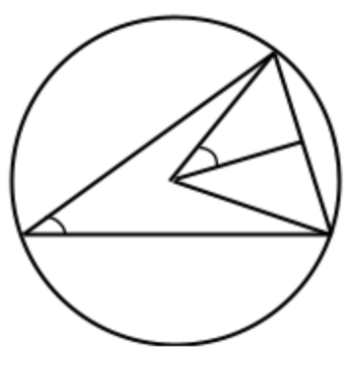
\includegraphics[width=0.4\linewidth]{Geometry/Content/42.png}
	
}

Сначала в самом общем виде докажем важную теорему $-$ теорему синусов.  Пусть в $\Delta ABC$, $\angle C = \alpha$, $AB=a$, а точка $O$ $-$ центр описанной около треугольника окружности радиуса $R$. Рассмотрим $\Delta OAB$. Т.к. $OA=OB+R$, этот треугольник равнобедренный и его высота $OD \perp AB$ является биссектрисой и медианой. Угол $AOB$ $-$ центральный, он вдвое больше вписанного угла $С$, опирающегося на ту же дугу окружности. Поэтому $\Delta OAD$ $-$ прямоугольный, а $\angle AOD=\alpha$, так что $\frac{a}{2}=R\sin{\alpha}$ или $\frac{a}{\sin{\alpha}}=2R$. Таким образом, в треугольнике отношение стороны к синусу противолежащего угла есть величина постоянная, равная $2R$. Это справедливо для  каждой стороны и противолежащего ей угла. Если стороны треугольника равны $a$, $b$, $c$, а противолежащие углы $A$, $B$, $C$, то 
\[
\frac{a}{\sin{A}}=\frac{b}{\sin{B}}=\frac{c}{\sin{C}}=2R.
\]
Эта теорема очень часто используется при решении геометрических задач. В нашей задаче $R = \frac{AB}{2\sin{30^\circ}}=AB=3$. \newline \null \hspace*{\fill} Ответ: 3.

\textbf{2138-2142} $-$ аналогичные задачи.

\textbf{2143.} Если четырехугольник вписан в окружность, то его противоположные углы опираются на дуги, дополняющие друг друга до полной окружности, т.е. их сумма равна $360^\circ$. Это означает, что противоположные углы в сумме составляют $180^\circ$. Тогда $\angle = 180^\circ - 46^\circ=134^\circ$. \newline \null \hspace*{\fill} Ответ: 134.

\textbf{2144, 2145} $-$ аналогичные задачи.

\textbf{2146.}

{\centering 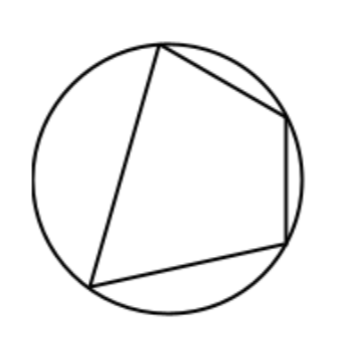
\includegraphics[width=0.35\linewidth]{Geometry/Content/43.png}
	
}

Угол $B$ опирается на сумму дуг $CD$ и $DA$, т.е. на дугу, градусная величина которой равна $90^\circ+145^\circ=235^\circ$; этот угол равен $\linebreak \frac{235^\circ}{2}=117,5^\circ$. \newline \null \hspace*{\fill} Ответ: 117,5.

\textbf{2147} $-$ аналогичная задача.

\textbf{2149.}  Поскольку $1+4+15+16=36$, нетрудно сообразить, что угол $A$ опирается на дугу $BCD$, градусная мера которой составляет $\frac{4+15}{36}\cdot360^\circ=190^\circ$, и равен $\frac{190^\circ}{2}=95^\circ$. \newline \null \hspace*{\fill} Ответ: 95.

\textbf{2148, 2150} $-$ аналогичные задачи.

\textbf{2151.}

{\centering 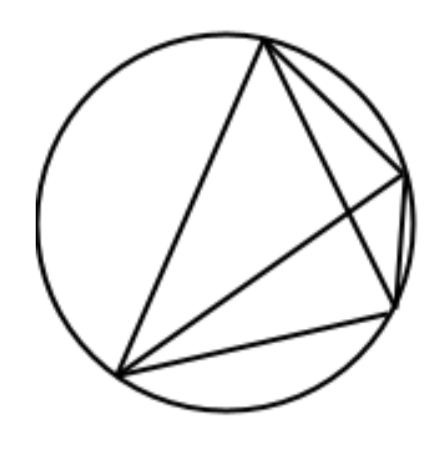
\includegraphics[width=0.35\linewidth]{Geometry/Content/44.png}
	
}

Угол $\angle DBC = \angle CAD = 38^\circ$, т.к. они опираются на одну и ту же дугу. Тогда $\angle ABD = \angle ABC - \angle DBC = 48^\circ - 38^\circ=10^\circ$. \newline \null \hspace*{\fill} Ответ: 10.

\textbf{2152, 2153} $-$ аналогичные задачи.

\textbf{2154.} Сумма данных двух углов не равна $180^\circ$, следовательно, эти углы не противоположные, а смежные. Значит, меньшему из этих углов соответствует больший противоположны угол, который равен $180^\circ-25^\circ=155^\circ$.\newline \null \hspace*{\fill} Ответ: 155.

\textbf{2155, 2156} $-$ аналогичные задачи.

\textbf{2157.} Из заданного соотношения углов следует, что все 4 последовательных угла  можно записать в виде: $x$, $13x$, $17x$, $y$. Но тогда $x+17x=13x+y$, откуда $y=5x$. Следовательно, градусная мера угла $D$ равна
\[
\frac{5x}{x+13x+17x+5x}\cdot360^\circ=50^\circ.
\]\null \hspace*{\fill} Ответ: 50.

\textbf{2158, 2159} $-$ аналогичные задачи.

\textbf{2160.} Пусть $\alpha$ $-$ вписанный угол, тогда центральный угол равен $2\alpha$. По условию задачи $2\alpha - \alpha = 45^\circ$, т.е. $\alpha = 45^\circ$. \newline \null \hspace*{\fill} Ответ: 45.

\textbf{2161, 2162} $-$ аналогичные задачи.

\textbf{2163.} Градусная мера дуги равна $\frac{5}{36}\cdot360^\circ=50^\circ$. Вписанный угол равен $\frac{50^\circ}{2} = 25^\circ$. \newline \null \hspace*{\fill} Ответ: 25.

\textbf{2164, 2165} $-$ аналогичные задачи.

\textbf{2166.} Градусная мера дуги равна $\frac{20}{100}\cdot360^\circ=72^\circ$. Вписанный угол равен $\frac{72^\circ}{2} = 36^\circ$. \newline \null \hspace*{\fill} Ответ: 36.

\textbf{2167, 2168} $-$ аналогичные задачи.

\textbf{2169.}

{\centering 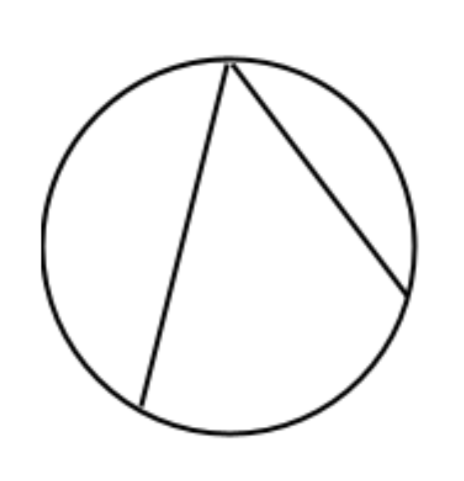
\includegraphics[width=0.35\linewidth]{Geometry/Content/45.png}
	
}

Из условия задачи следует, что дуги $AC$ и $BC$ расположены по разные стороны от точки $C$. Тогда дуга $AB$ составляет $360^\circ-\linebreak-165^\circ-55^\circ=140^\circ$, а угол $ACB=\frac{140^\circ}{2}=70^\circ$. \newline \null \hspace*{\fill} Ответ: 70.

\textbf{2170, 2171} $-$ аналогичные задачи.

\textbf{2172.}

{\centering 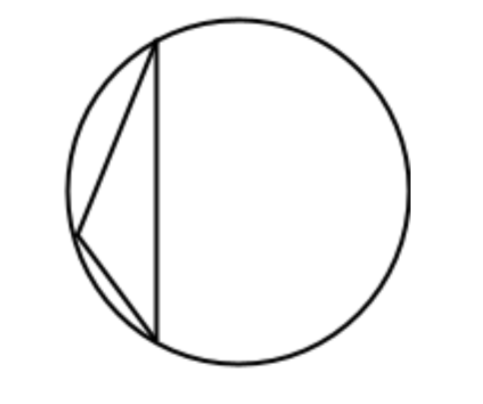
\includegraphics[width=0.35\linewidth]{Geometry/Content/46.png}
	
}

Градусная мера дуги $AC$, на которую опирается угол $ABC$, равна
$\frac{15}{1+2+15}\cdot360^\circ=300^\circ$. Угол $ABC$ равен $\frac{300^\circ}{2}=150^\circ$. \newline \null \hspace*{\fill} Ответ: 150.

\textbf{2173, 2174} $-$ аналогичные задачи.

\textbf{2175.}

{\centering 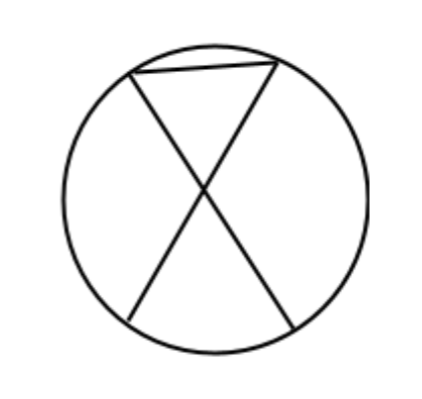
\includegraphics[width=0.35\linewidth]{Geometry/Content/47.png}
	
}

Дуга $AB$, на которую опирается угол $ACB$, равна $2\cdot69^\circ=138^\circ$. Т.к. дуга $BAD$ стягивает диаметр $BD$, то дуга $AD$ равна $180^\circ-\linebreak-138^\circ=42^\circ$. Центральный угол $AOD$ также равен $42^\circ$. \newline \null \hspace*{\fill} Ответ: 42.

\textbf{2176, 2177} $-$ аналогичные задачи.

\textbf{2178.}

{\centering 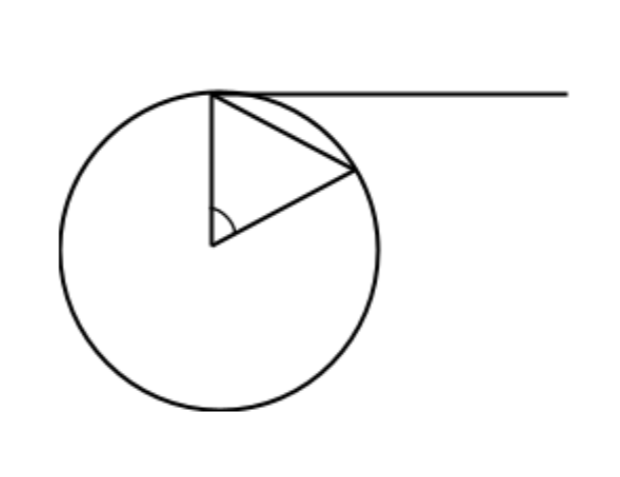
\includegraphics[width=0.35\linewidth]{Geometry/Content/48.png}
	
}

Сначала дадим ответ на вопрос: чему равен угол между касательной к окружности $AB$ и хордой $BC$, проведенной через точку касания $B$? Проведем из центра окружности точки $O$ радиусы $OB$ и $OC$ к концам хорды и обозначим $\angle BOC=\alpha$. Тогда дуга окружности $BC$, заключенная между касательной и хордой, также равна $\alpha$. Т.к. радиус, проведенный в точку касания, перпендикулярен касательной, то угол $OBA$ равен $90^\circ$. Окончательно получаем: 
\[
\angle ABC = 90^\circ - \angle OBC = 90^\circ-\frac{180^\circ-\alpha}{2}=\frac{\alpha}{2}.
\]
Таким образом, угол между касательной и хордой, проведенной через точку касания, измеряется половиной дуги окружности, заключенной между касательной и хордой. 

Это общий результат. В нашем случае дуга равна $6^\circ$, следовательно, угол $ABC$ равен $3^\circ$. \newline \null \hspace*{\fill} Ответ: 3.

\textbf{2179, 2180} $-$ аналогичные задачи.

\textbf{2181.} Т.к. $OA \perp AC$ и $OB \perp BC$, то $\angle AOB = 360^\circ - 2\cdot90^\circ - \angle C = \linebreak =180^\circ-79^\circ=101^\circ.$ \newline \null \hspace*{\fill} Ответ: 101.

\textbf{2182, 2183} $-$ аналогичные задачи.

\textbf{2184.} По аналогии с задачей \textbf{2181} угол $AOB$ равен $180^\circ-2^\circ=\linebreak=178^\circ$. Тогда из равнобедренного треугольника $AOB$ получаем:
\[
\angle ABO=\frac{180^\circ-178^\circ}{2}=1^\circ.
\] \null \hspace*{\fill} Ответ: 1.

\textbf{2185, 2186} $-$ аналогичные задачи.

\textbf{2187.}

{\centering 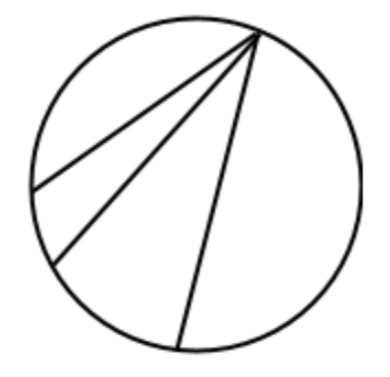
\includegraphics[width=0.35\linewidth]{Geometry/Content/49.png}
	
}

 Угол $ADB$ равен $\frac{128^\circ}{2}=64^\circ$. угол $ADC$ равен $\frac{48^\circ}{2}=24^\circ$, так что $\angle CDB = 64^\circ - 24^\circ=40^\circ.$ \newline \null \hspace*{\fill} Ответ: 40.

\textbf{2188, 2189} $-$ аналогичные задачи.

\textbf{2190.}

{\centering 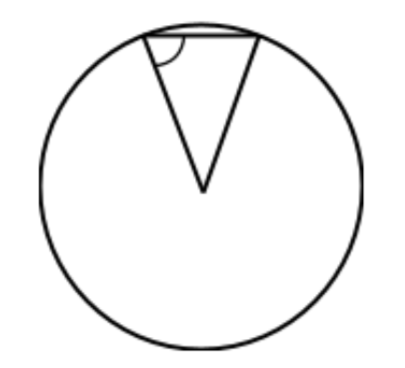
\includegraphics[width=0.35\linewidth]{Geometry/Content/50.png}
	
}

Пусть $AB$ $-$ сторона правильного n-угольника, вписанного в \newline окружность. Тогда центральный угол $AOB$ равен $\frac{360\circ}{n}$, а в треугольнике $AOB$:
\begin{gather*}
	\angle OAB = \frac{180^\circ-\frac{360^\circ}{n}}{1}=75^\circ, \; 180^\circ-\frac{360^\circ}{n}=150^\circ, \\ \frac{360^\circ}{n}=30^\circ,\;  n =12.
\end{gather*} \null \hspace*{\fill} Ответ: 12.

\textbf{2191, 2192} $-$ аналогичные задачи.

\textbf{2193.} $S=\pi R^2= \frac{625}{\pi}$, $(\pi R)^2 = 625$, $\pi R = 25$, $C = 2\pi R = 50.$ \newline \null \hspace*{\fill} Ответ: 50.

\textbf{2194, 2195} $-$ аналогичные задачи.

\textbf{2196.} Если $\alpha = 90^\circ$ $-$ центральный угол сектора, то площадь сектора $S_c=\pi R^2 \cdot \frac{\alpha}{360}=\pi \cdot \frac{1600}{\pi}\cdot \frac{90}{360} =400.$ \newline \null \hspace*{\fill} Ответ: 400.

\textbf{2197, 2198} $-$ аналогичные задачи.

\textbf{2199.} Если длина дуги сектора равна $L$, то площадь сектора в $\frac{L}{2\pi R}$ раз меньше площади круга, т.е. она равна $\pi R^2 \cdot \frac{L}{2\pi R} = \frac{RL}{2}=\linebreak\;=\;\;\frac{24\cdot 3}{2}=36.$ \newline \null \hspace*{\fill} Ответ: 36.

\textbf{2200, 2201} $-$ аналогичные задачи.

\textbf{2202.} $S = rp = \frac{rP}{2}=8.$ \newline \null \hspace*{\fill} Ответ: 8.

\textbf{2203-2209} $-$ аналогичные задачи.

\textbf{2210.}  Формула $S=rp=\frac{rP}{2}$ справедлива для любого выпуклого многоугольника, описанного около окружности. Так что $P=\frac{2S}{r}=29.$ \newline \null \hspace*{\fill} Ответ: 29.

\textbf{2211-2213} $-$ аналогичные задачи.

\textbf{2214.} $S_k=\pi(R^2-r^2)=\pi\left( \frac{81}{\pi} - \frac{25}{\pi}\right)=56.$ \newline \null \hspace*{\fill} Ответ: 56.

\textbf{2215- 2217} $-$ аналогичные задачи.

\textbf{2218.} См. решение задачи \textbf{2199} $S_c = \frac{RL}{2}$, $L=\frac{2S_c}{R}=15.$ \newline \null \hspace*{\fill} Ответ: 15.